\documentclass[../Head/Main.tex]{subfiles}
\begin{document}
\subsection{Estimate for path lengths}
\label{subsec:est_path_length}
The purpose of this test was to find an estimate for the distances between the rooms in order to have a distance punishment for the Q-learning.
\subsubsection{Description of test}
This test was conducted using Geogebra a cas tool for geometry and algebra. An image of the environment "bigworld" was loaded into the program. The width of the image was set to 8.4 cm.\par 
Based on this lines was drawn by hand between the centroids of the rooms navigating any obstacles. This can be seen on figure \ref{fig:geogebra}.
\begin{figure}[H]
	\centering
	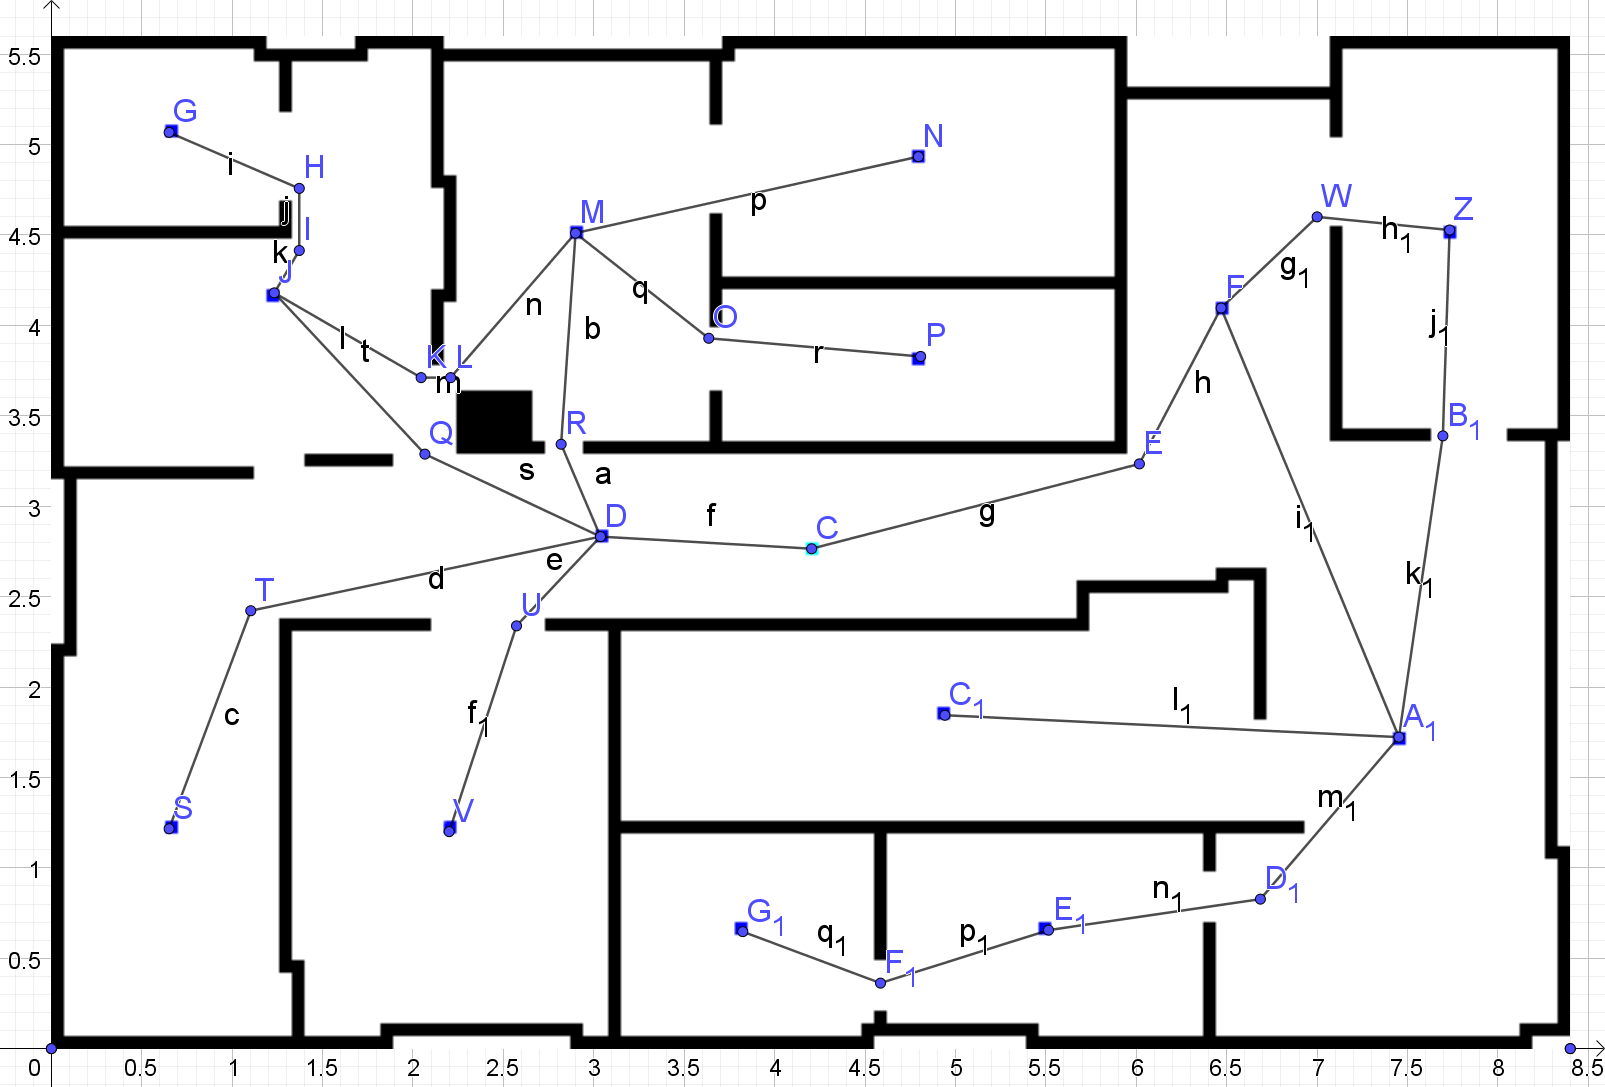
\includegraphics[width=0.6\textwidth]{map_medium_geogebra}
	\caption{Illustration of paths in geogebra}
	\label{fig:geogebra}
\end{figure}
Geogebra calculates the length of each line. Based on this the total path length from one room to another was found. This can be seen in table gegegepgkek
\subsubsection{Test parameters}
\begin{tabular}{l r}
	- World used                & bigworld\\	
	- Length of world           & 8.4 cm\\
\end{tabular}

\subsubsection{Data}
\begin{table}[H]
	\centering
	\begin{tabular}{l r c l r}
		\hline
		\multicolumn{5}{l}{\textbf{Distribution of marbles}}  			\\ \hline
		Distance from room 1 to 2   & -2.78 & &
		Distance from room 2 to 3   & -4.32\\
		Distance from room 2 to 6   & -4.58 & &
		Distance from room 3 to 4   & -3.88\\
		Distance from room 3 to 5   & -4.24 & &
		Distance from room 3 to 6   & -3.46\\
		Distance from room 6 to 7   & -6.54 & &
		Distance from room 6 to 8   & -3.76\\
		Distance from room 7 to 9   & -8.02 & &
		Distance from room 9 to 10  & -2.94\\
		Distance from room 9 to 11  & -5.14 & &
		Distance from room 10 to 11 & -5.64\\
		Distance from room 11 to 12 & -5.02 & &
		Distance from room 11 to 13 & -4.72\\
		Distance from room 13 to 14 & -3.56 & & \\						\hline
	\end{tabular}
	\caption{Distances between rooms}
	\label{tab:dist_geogebra}
\end{table}

\end{document}